\documentclass[a4paper,12pt]{article}

%%%%%%%% CREATE DOCUMENT STRUCTURE %%%%%%%%
%% Language and font encodings
\usepackage[english]{babel}
\usepackage[utf8x]{inputenc}
\usepackage[T1]{fontenc}

%% Sets page size and margins
\usepackage[a4paper,top=2.5cm,bottom=2.5cm,left=2cm,right=2cm,marginparwidth=1.75cm]{geometry}

%% Useful packages
\usepackage{amsmath}
\usepackage{graphicx}
\usepackage[colorinlistoftodos]{todonotes}
\usepackage[colorlinks=true, allcolors=blue]{hyperref}
\usepackage{caption}
\usepackage{subcaption}
\usepackage{sectsty}
\usepackage{float}
\usepackage{titling}
\usepackage{booktabs}
\usepackage{tabularx}
\usepackage{enumitem}
\usepackage{listings}
\usepackage[square,sort,comma,numbers]{natbib}
\usepackage{xcolor}

%% TikZ for native, high-quality vector diagrams
\usepackage{tikz}
\usetikzlibrary{shapes.geometric, shapes.misc, arrows.meta, positioning, calc, fit, backgrounds}

%% Color definitions
\definecolor{navyblue}{RGB}{15, 23, 42}
\definecolor{accentblue}{RGB}{37, 99, 235}
\definecolor{accentteal}{RGB}{13, 148, 136}

%% TikZ Styling Matching Uploaded DFD Reference Architecture
\tikzset{
    entity3D/.style={
        draw=black, line width=1pt, fill=white,
        text centered, font=\bfseries\small,
        preaction={fill=black, transform canvas={xshift=4pt, yshift=-4pt}}
    },
    usecase/.style={
        ellipse, draw=accentblue, fill=blue!5,
        minimum width=3.2cm, minimum height=0.75cm, text centered, font=\footnotesize\bfseries
    },
    actorNode/.style={
        rectangle, rounded corners=3pt, draw=navyblue, fill=gray!15,
        minimum width=2.0cm, minimum height=0.85cm, text centered, font=\small\bfseries
    },
    dfdArrow/.style={
        -{Latex[length=2.5mm]}, draw=black, line width=0.8pt
    },
    dfdBiArrow/.style={
        {Latex[length=2.5mm]}-{Latex[length=2.5mm]}, draw=black, line width=0.8pt
    },
    wireframeBox/.style={
        rectangle, draw=navyblue, fill=white, line width=0.8pt,
        rounded corners=4pt
    }
}

%% Section heading styling
\sectionfont{\color{navyblue}}
\subsectionfont{\color{accentteal}}
\subsubsectionfont{\color{accentblue}}

%%%%%%%% DOCUMENT %%%%%%%%
\begin{document}

%%%% Title Page
\begin{titlepage}
\newcommand{\HRule}{\rule{\linewidth}{0.5mm}} 							
\centering
 
% University Logo (Fallback if image not present)
\IfFileExists{images/Adamas_logo.png}{
    \includegraphics[width=0.45\textwidth]{images/Adamas_logo.png}\\[0.8cm]
}{
    \vspace*{0.5cm}
    \textsc{\Huge \textbf{ADAMAS UNIVERSITY}}\\[0.8cm]
}

\textsc{\LARGE Department of Computer Science \& Engineering}\\[0.5cm]

% Document info
\textsc{\Large SUBJECT: Software Engineering}\\[0.2cm]
\textsc{\large COURSE CODE: CSE11117}\\[0.8cm] 										
\HRule \\[0.5cm]
{ \huge \bfseries Assignment: Course Registration Management System}\\[0.4cm]
{ \large \bfseries Software Requirements Specification (SRS) \& System Architecture}\\[0.3cm]
\HRule \\[1.5cm]

\begin{minipage}{0.45\textwidth}
    \begin{flushleft} \large
        \emph{Name:}\\
        \textbf{Aditya Chatterjee}
    \end{flushleft}
\end{minipage}
\begin{minipage}{0.45\textwidth}
    \begin{flushright} \large
        \emph{Academic Year:}\\
        2025--2026
    \end{flushright}
\end{minipage}

\vfill
{\large \today}\\[1cm]
\end{titlepage}
\newpage

%%%% SECTIONS    
\section*{ABSTRACT}
Educational institutions need centralised software programmes if they are to make the switch to a digital infrastructure. The present project involves the introduction of a comprehensive Course Registration System in order to update the process of academic enrollment. Traditional manual registration is usually suffering from scheduling conflicts, data redundancy, and mistakes caused by humans. Through moving to a dynamic digital environment, this software offers a solid platform enabling smooth and real-time interaction between students and administrators.
\\\\
Because of its modular design, the system guarantees data consistency and usability. The student interface enables secure authentication, allows students to browse courses, manage their schedule, and carry out add-and-drop operations. At the same time, an administrative console provides staff with the means to manage the course catalogue, assign faculty members, and modify batch. Moreover, a backend validation engine automatically checks student prerequisites, enforces credit limits, and stops scheduling conflicts before enrollments are finalised.
\\\\
In the end, introducing this automated system will greatly cut down on administrative work and lead to a more efficient use of institutional resources. Since it gets rid of the bottlenecks associated with manual data entry, the system guarantees data security and enhances the overall user experience. The new application offers a scalable and maintainable base which can deal with future academic growth.

\newpage
\tableofcontents
\newpage

\section{Introduction}

\subsection{Purpose}
The purpose of this Software Requirements Specification (SRS) document is to specify the detailed functional and non-functional requirements, software development process models, architectural patterns, and behavioral models for \textbf{My Student Academia}. This document serves as the foundational engineering contract across software developers, quality assurance teams, academic reviewers, and administrative stakeholders.

\subsection{Document Conventions}
This document is prepared in accordance with the \textbf{IEEE Std 830-1998} standard. The following typographic conventions are utilized:
\begin{itemize}[leftmargin=1.2cm]
    \item \textbf{Boldface:} Used for actor names, core architectural components, database models, and critical business rules.
    \item \texttt{Monospace:} Denotes database attributes, RESTful API paths, and programmatic variables.
    \item \textit{Italics:} Highlights lifecycle states (e.g., \textit{ENROLLED}, \textit{WAITING}, \textit{DROPPED}) and external document references.
    \item \textbf{Priority Classification:} Requirements are classified as Essential ($E$), Desirable ($D$), or Optional ($O$).
\end{itemize}

\subsection{Intended Audience and Reading Suggestions}
This document is organized for multiple reader groups:
\begin{itemize}[leftmargin=1.2cm]
    \item \textbf{Academic Evaluators \& Faculty:} Recommended to review Section 1 (Introduction), Section 2.1 (Product Perspective, SDLC Process Model Analysis), Section 2.2 (Product Functions), and Section 4 (System Features).
    \item \textbf{Software Architects \& Developers:} Should focus on Section 2.1 (3-Tier Layered Architecture, DFD Levels 0, 1, 2), Section 3 (External Interfaces), and Section 4 (Functional Requirements).
    \item \textbf{Quality Assurance (QA) Engineers:} Should review Section 2.1 (DFD Level 2 Validation Flow), Section 3.4 (Communications Interfaces), and Section 4 (Stimulus/Response Sequences) for test case formulation.
\end{itemize}

\subsection{Product Scope}
\textbf{My Student Academia} is an automated, web-based Academic Course Registration and Management System. The software centralizes multi-departmental course offerings, automates prerequisite graph validation, enforces maximum semester credit ceilings (capped at 24 credits per semester), and manages real-time section capacities with automated FIFO waitlist queues. It provides dedicated role-based interfaces for \textbf{Students}, \textbf{Faculty Instructors}, and \textbf{Academic Administrators}. \textit{(Note: Timetable scheduling matrix logic was intentionally excluded to preserve maximum modularity and focus strictly on course registration workflows)}.

\subsection{References}
\begin{enumerate}[leftmargin=1.2cm]
    \item IEEE Std 830-1998, \textit{IEEE Recommended Practice for Software Requirements Specifications}, IEEE Computer Society.
    \item IEEE Std 1016-2009, \textit{IEEE Standard for Information Technology---Systems Design---Software Design Descriptions}.
    \item Ian Sommerville, \textit{Software Engineering}, 10th Edition, Pearson, 2015.
    \item Roger S. Pressman, \textit{Software Engineering: A Practitioner's Approach}, 8th Edition, McGraw-Hill, 2014.
\end{enumerate}

\section{Overall Description}

\subsection{Product Perspective}
\textbf{My Student Academia} is a standalone, full-stack 3-Tier Layered Client-Server software application. It replaces legacy manual enrollment workflows with a modern, high-performance web architecture:

\begin{figure}[H]
\centering
\resizebox{0.95\linewidth}{!}{
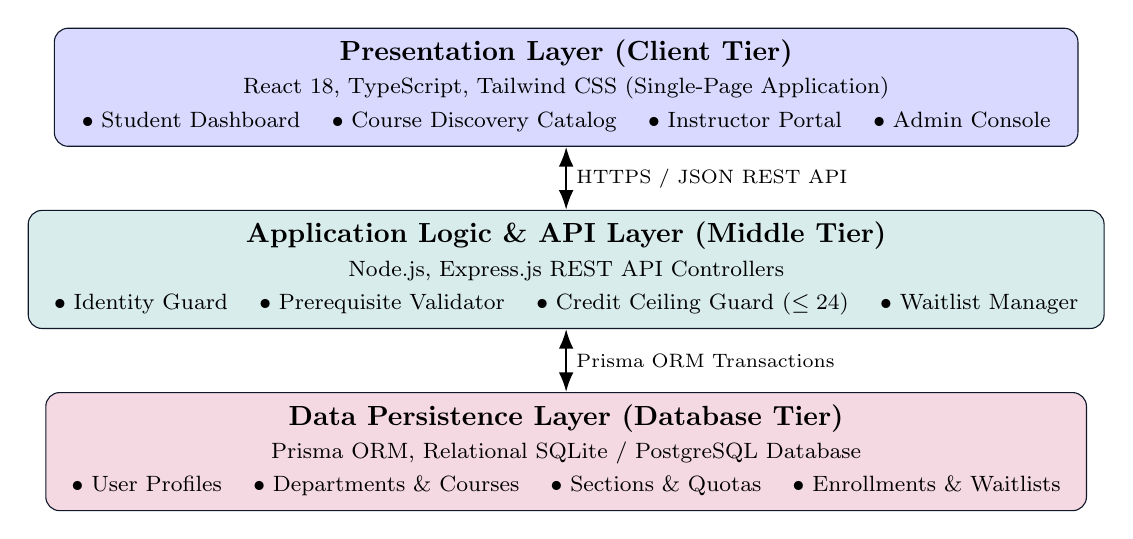
\begin{tikzpicture}[node distance=1.1cm, auto]
    \node (tier1) [rectangle, rounded corners=5pt, draw=navyblue, fill=blue!15, minimum width=13cm, minimum height=1.1cm] {
        \begin{tabular}{c}
            \textbf{Presentation Layer (Client Tier)}\\
            \footnotesize React 18, TypeScript, Tailwind CSS (Single-Page Application)\\
            \footnotesize $\bullet$ Student Dashboard \quad $\bullet$ Course Discovery Catalog \quad $\bullet$ Instructor Portal \quad $\bullet$ Admin Console
        \end{tabular}
    };
    
    \node (tier2) [rectangle, rounded corners=5pt, draw=navyblue, fill=teal!15, minimum width=13cm, minimum height=1.1cm, below=0.8cm of tier1] {
        \begin{tabular}{c}
            \textbf{Application Logic \& API Layer (Middle Tier)}\\
            \footnotesize Node.js, Express.js REST API Controllers\\
            \footnotesize $\bullet$ Identity Guard \quad $\bullet$ Prerequisite Validator \quad $\bullet$ Credit Ceiling Guard ($\le 24$) \quad $\bullet$ Waitlist Manager
        \end{tabular}
    };
    
    \node (tier3) [rectangle, rounded corners=5pt, draw=navyblue, fill=purple!15, minimum width=13cm, minimum height=1.1cm, below=0.8cm of tier2] {
        \begin{tabular}{c}
            \textbf{Data Persistence Layer (Database Tier)}\\
            \footnotesize Prisma ORM, Relational SQLite / PostgreSQL Database\\
            \footnotesize $\bullet$ User Profiles \quad $\bullet$ Departments \& Courses \quad $\bullet$ Sections \& Quotas \quad $\bullet$ Enrollments \& Waitlists
        \end{tabular}
    };
    
    \draw [dfdBiArrow] (tier1) -- node[right, font=\scriptsize] {HTTPS / JSON REST API} (tier2);
    \draw [dfdBiArrow] (tier2) -- node[right, font=\scriptsize] {Prisma ORM Transactions} (tier3);
\end{tikzpicture}
}
\caption{3-Tier Layered Architecture of My Student Academia}
\end{figure}

\subsubsection{Software Engineering Process Model Analysis}
The development methodology governs system reliability, architectural refinement, and risk mitigation. The following classical process models were evaluated:

\begin{table}[H]
\centering
\small
\renewcommand{\arraystretch}{1.3}
\begin{tabularx}{\textwidth}{>{\bfseries\raggedright\arraybackslash}p{2.6cm} >{\raggedright\arraybackslash}p{4.0cm} >{\raggedright\arraybackslash}p{4.0cm} >{\raggedright\arraybackslash}X}
\toprule
\textbf{SDLC Model} & \textbf{Core Philosophy} & \textbf{Engineering Strengths} & \textbf{Suitability for this Project} \\
\midrule
Waterfall Model & Linear-sequential phases (Requirements $\to$ Design $\to$ Implementation $\to$ Verification). & Clear milestones and straightforward project tracking. & \textbf{Unsuitable:} Highly rigid; prohibits early prototyping and iterative rule changes. \\
\addlinespace
Spiral Model & Risk-driven iterative cycles combining Waterfall milestones with formal risk analysis. & Strong risk mitigation for high-risk mission-critical systems. & \textbf{Sub-optimal:} Excessive management overhead for a web-based educational system. \\
\addlinespace
Agile Incremental Iterative Model & Decomposes the system into small functional increments delivered in rapid sprint cycles. & Continuous feedback, early working software, adaptive schema changes, rapid validation. & \textbf{Selected:} Optimal for developing role portals, API contracts, and complex validation rules in parallel. \\
\bottomrule
\end{tabularx}
\caption{Comparative Analysis of Software Development Process Models}
\end{table}

\begin{figure}[H]
\centering
\resizebox{0.92\linewidth}{!}{
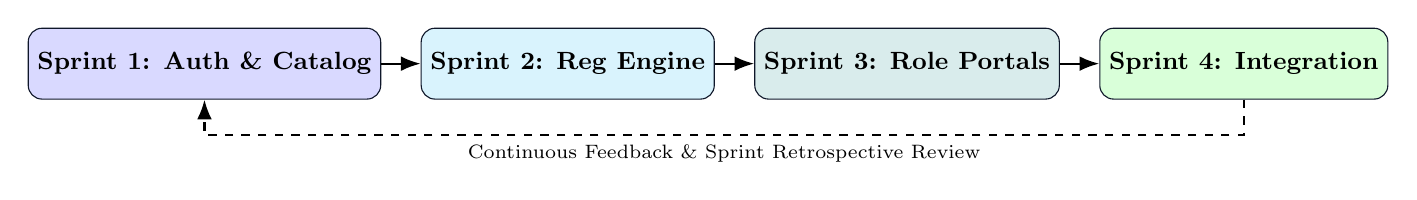
\begin{tikzpicture}[node distance=0.4cm, auto]
    \node (s1) [rectangle, rounded corners=5pt, draw=navyblue, fill=blue!15, minimum width=2.8cm, minimum height=0.9cm, font=\small\bfseries] {Sprint 1: Auth \& Catalog};
    \node (s2) [rectangle, rounded corners=5pt, draw=navyblue, fill=cyan!15, minimum width=2.8cm, minimum height=0.9cm, right=0.5cm of s1, font=\small\bfseries] {Sprint 2: Reg Engine};
    \node (s3) [rectangle, rounded corners=5pt, draw=navyblue, fill=teal!15, minimum width=2.8cm, minimum height=0.9cm, right=0.5cm of s2, font=\small\bfseries] {Sprint 3: Role Portals};
    \node (s4) [rectangle, rounded corners=5pt, draw=navyblue, fill=green!15, minimum width=2.8cm, minimum height=0.9cm, right=0.5cm of s3, font=\small\bfseries] {Sprint 4: Integration};
    
    \draw [dfdArrow] (s1) -- (s2);
    \draw [dfdArrow] (s2) -- (s3);
    \draw [dfdArrow] (s3) -- (s4);
    
    \draw [dfdArrow, dashed] (s4.south) -- ++(0,-0.45) -| node[pos=0.25, below, font=\scriptsize] {Continuous Feedback \& Sprint Retrospective Review} (s1.south);
\end{tikzpicture}
}
\caption{Agile Incremental Iterative Sprint Workflow}
\end{figure}

\newpage
\subsubsection{Data Flow Diagrams (DFD)}

\paragraph{DFD Level 0: Context Diagram}
The Level 0 Context Diagram captures high-level data exchanges between external entities and the core system with dedicated, non-overlapping label channels.

\begin{figure}[H]
\centering
\resizebox{0.95\linewidth}{!}{
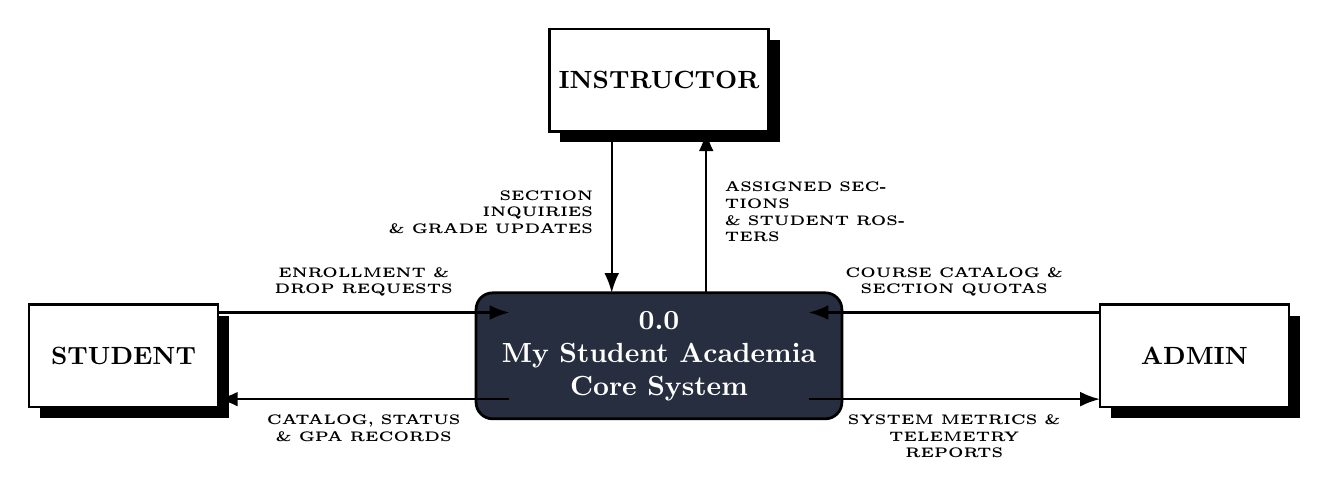
\begin{tikzpicture}[auto]
    % Center System Box
    \node (sys) [rectangle, rounded corners=6pt, draw=black, line width=1pt, fill=navyblue!90, text=white, minimum width=3.8cm, minimum height=1.6cm] at (0,0) {
        \begin{tabular}{c}
            \textbf{0.0}\\
            \textbf{My Student Academia}\\
            \textbf{Core System}
        \end{tabular}
    };
    
    % External Entity Boxes (3D Shadow Box Style)
    \node (stu) [entity3D, minimum width=2.4cm, minimum height=1.3cm] at (-6.8, 0) {STUDENT};
    \node (inst) [entity3D, minimum width=2.6cm, minimum height=1.3cm] at (0, 3.5) {INSTRUCTOR};
    \node (admin) [entity3D, minimum width=2.4cm, minimum height=1.3cm] at (6.8, 0) {ADMIN};
    
    % Student <-> System Arrows
    \draw [dfdArrow] (-5.6, 0.55) -- node[above=2pt, text width=2.8cm, align=center, font=\tiny\bfseries] {ENROLLMENT \&\\DROP REQUESTS} (-1.9, 0.55);
    \draw [dfdArrow] (-1.9, -0.55) -- node[below=2pt, text width=2.8cm, align=center, font=\tiny\bfseries] {CATALOG, STATUS\\\& GPA RECORDS} (-5.6, -0.55);
    
    % Instructor <-> System Arrows
    \draw [dfdArrow] (-0.6, 2.85) -- node[left=3pt, text width=2.6cm, align=right, font=\tiny\bfseries] {SECTION INQUIRIES\\\& GRADE UPDATES} (-0.6, 0.8);
    \draw [dfdArrow] (0.6, 0.8) -- node[right=3pt, text width=2.6cm, align=left, font=\tiny\bfseries] {ASSIGNED SECTIONS\\\& STUDENT ROSTERS} (0.6, 2.85);
    
    % Admin <-> System Arrows
    \draw [dfdArrow] (5.6, 0.55) -- node[above=2pt, text width=2.8cm, align=center, font=\tiny\bfseries] {COURSE CATALOG \&\\SECTION QUOTAS} (1.9, 0.55);
    \draw [dfdArrow] (1.9, -0.55) -- node[below=2pt, text width=2.8cm, align=center, font=\tiny\bfseries] {SYSTEM METRICS \&\\TELEMETRY REPORTS} (5.6, -0.55);
\end{tikzpicture}
}
\caption{DFD Level 0: Context Diagram}
\end{figure}

\newpage
\paragraph{DFD Level 1: Course Registration \& Academic Management}
The Level 1 DFD decomposes the central system into Process 1 with wide, collision-free communication channels between all actors and data stores.

\begin{figure}[H]
\centering
\resizebox{0.95\linewidth}{!}{
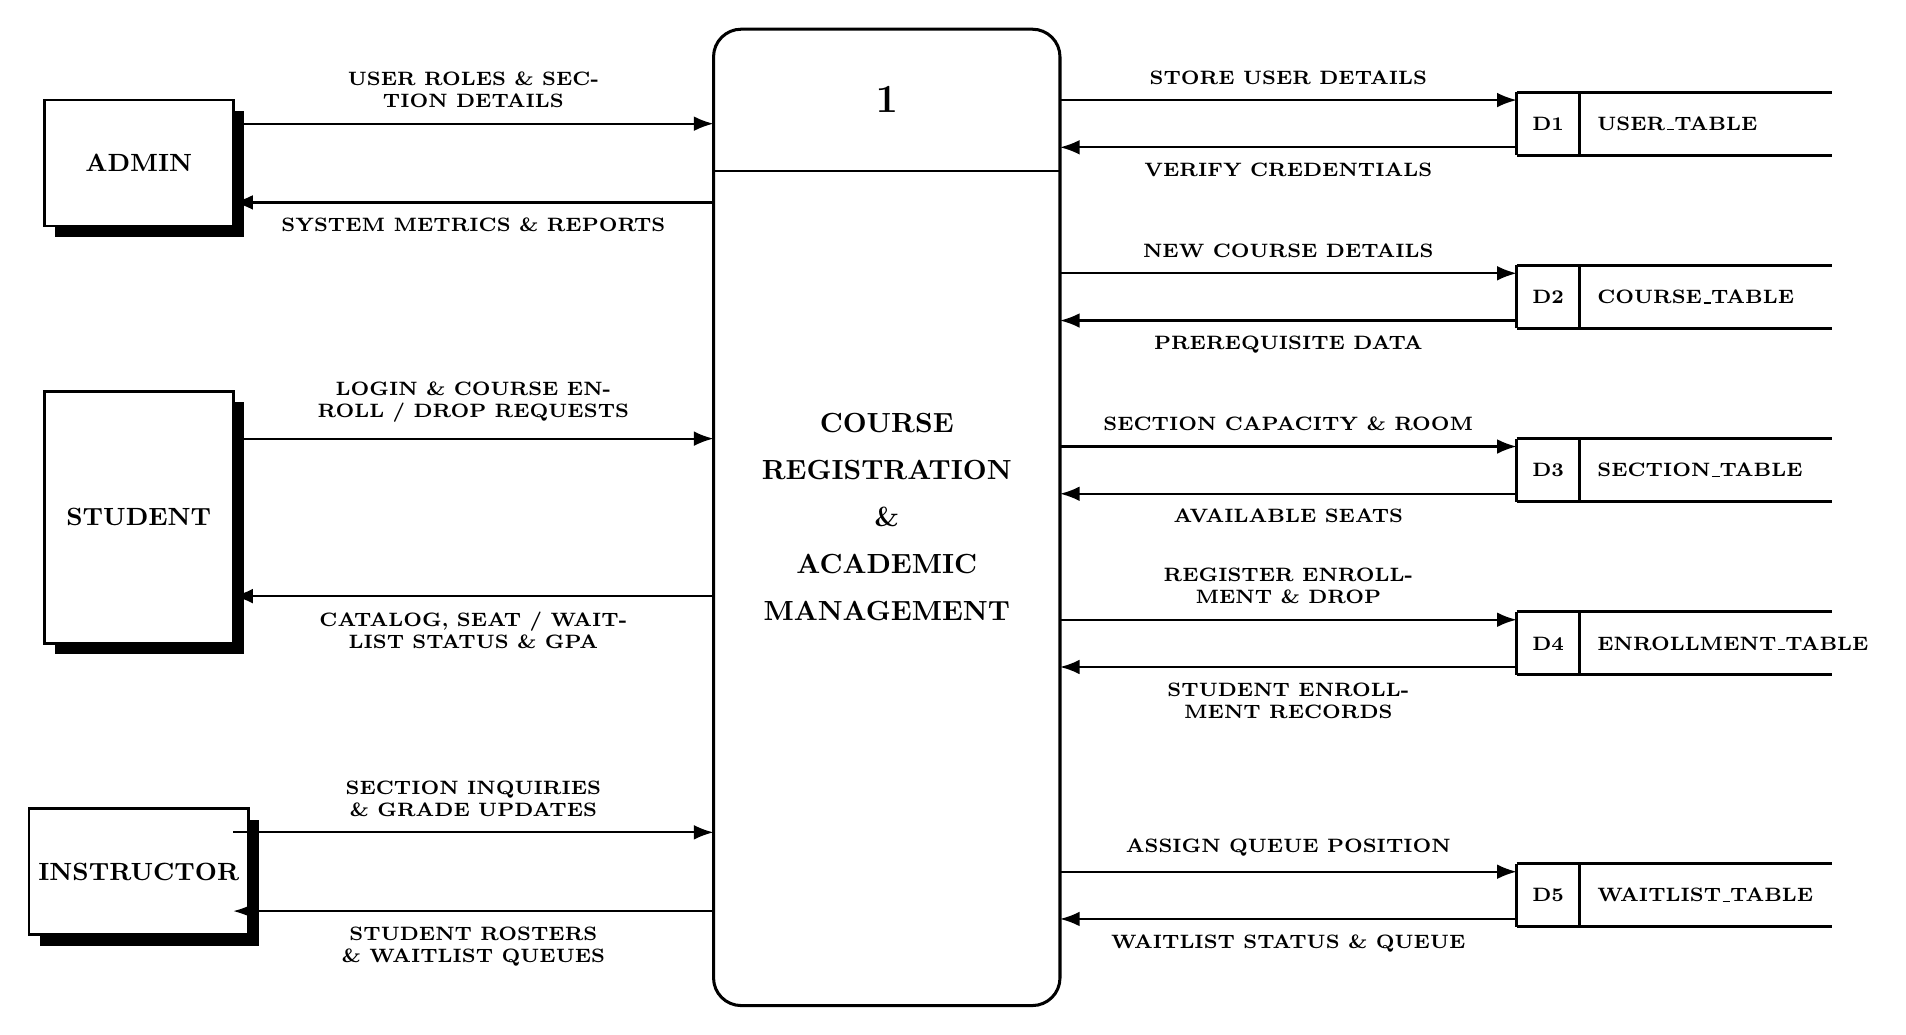
\begin{tikzpicture}[auto]
    % Central Process 1 Box (Divided Header)
    \draw[draw=black, line width=1.1pt, fill=white, rounded corners=10pt] (-2.2, -6.2) rectangle (2.2, 6.2);
    \draw[line width=1pt] (-2.2, 4.4) -- (2.2, 4.4);
    \node[font=\bfseries\Large] at (0, 5.3) {1};
    \node[font=\bfseries\normalsize, align=center] at (0, 0.0) {
        \textbf{COURSE}\\[5pt]
        \textbf{REGISTRATION}\\[5pt]
        \textbf{\&}\\[5pt]
        \textbf{ACADEMIC}\\[5pt]
        \textbf{MANAGEMENT}
    };

    % External Entities on the Left (Positioned at x = -9.5)
    \node (admin) [entity3D, minimum width=2.4cm, minimum height=1.6cm] at (-9.5, 4.5) {ADMIN};
    \node (student) [entity3D, minimum width=2.4cm, minimum height=3.2cm] at (-9.5, 0.0) {STUDENT};
    \node (instructor) [entity3D, minimum width=2.4cm, minimum height=1.6cm] at (-9.5, -4.5) {INSTRUCTOR};

    % Data Stores on the Right (Positioned at x = 8.0)
    % D1: USER_TABLE
    \draw[line width=1pt] (8.0, 5.4) -- (12.0, 5.4);
    \draw[line width=1pt] (8.0, 4.6) -- (12.0, 4.6);
    \draw[line width=1pt] (8.0, 4.6) -- (8.0, 5.4);
    \draw[line width=1pt] (8.8, 4.6) -- (8.8, 5.4);
    \node[font=\bfseries\scriptsize] at (8.4, 5.0) {D1};
    \node[font=\bfseries\scriptsize, anchor=west] at (8.9, 5.0) {USER\_TABLE};

    % D2: COURSE_TABLE
    \draw[line width=1pt] (8.0, 3.2) -- (12.0, 3.2);
    \draw[line width=1pt] (8.0, 2.4) -- (12.0, 2.4);
    \draw[line width=1pt] (8.0, 2.4) -- (8.0, 3.2);
    \draw[line width=1pt] (8.8, 2.4) -- (8.8, 3.2);
    \node[font=\bfseries\scriptsize] at (8.4, 2.8) {D2};
    \node[font=\bfseries\scriptsize, anchor=west] at (8.9, 2.8) {COURSE\_TABLE};

    % D3: SECTION_TABLE
    \draw[line width=1pt] (8.0, 1.0) -- (12.0, 1.0);
    \draw[line width=1pt] (8.0, 0.2) -- (12.0, 0.2);
    \draw[line width=1pt] (8.0, 0.2) -- (8.0, 1.0);
    \draw[line width=1pt] (8.8, 0.2) -- (8.8, 1.0);
    \node[font=\bfseries\scriptsize] at (8.4, 0.6) {D3};
    \node[font=\bfseries\scriptsize, anchor=west] at (8.9, 0.6) {SECTION\_TABLE};

    % D4: ENROLLMENT_TABLE
    \draw[line width=1pt] (8.0, -1.2) -- (12.0, -1.2);
    \draw[line width=1pt] (8.0, -2.0) -- (12.0, -2.0);
    \draw[line width=1pt] (8.0, -2.0) -- (8.0, -1.2);
    \draw[line width=1pt] (8.8, -2.0) -- (8.8, -1.2);
    \node[font=\bfseries\scriptsize] at (8.4, -1.6) {D4};
    \node[font=\bfseries\scriptsize, anchor=west] at (8.9, -1.6) {ENROLLMENT\_TABLE};

    % D5: WAITLIST_TABLE
    \draw[line width=1pt] (8.0, -4.4) -- (12.0, -4.4);
    \draw[line width=1pt] (8.0, -5.2) -- (12.0, -5.2);
    \draw[line width=1pt] (8.0, -5.2) -- (8.0, -4.4);
    \draw[line width=1pt] (8.8, -5.2) -- (8.8, -4.4);
    \node[font=\bfseries\scriptsize] at (8.4, -4.8) {D5};
    \node[font=\bfseries\scriptsize, anchor=west] at (8.9, -4.8) {WAITLIST\_TABLE};

    % Admin Connections (Arrow span = 6.1cm, text width = 5.2cm -> Zero overlap)
    \draw [dfdArrow] (-8.3, 5.0) -- node[above=2pt, font=\scriptsize\bfseries, text width=5.2cm, align=center] {USER ROLES \& SECTION DETAILS} (-2.2, 5.0);
    \draw [dfdArrow] (-2.2, 4.0) -- node[below=2pt, font=\scriptsize\bfseries, text width=5.2cm, align=center] {SYSTEM METRICS \& REPORTS} (-8.3, 4.0);

    % Student Connections (Separated by 2.0cm vertical buffer -> Zero collision)
    \draw [dfdArrow] (-8.3, 1.0) -- node[above=2pt, font=\scriptsize\bfseries, text width=5.2cm, align=center] {LOGIN \& COURSE ENROLL / DROP REQUESTS} (-2.2, 1.0);
    \draw [dfdArrow] (-2.2, -1.0) -- node[below=2pt, font=\scriptsize\bfseries, text width=5.2cm, align=center] {CATALOG, SEAT / WAITLIST STATUS \& GPA} (-8.3, -1.0);

    % Instructor Connections (Arrow span = 6.1cm, text width = 5.2cm -> Zero overlap)
    \draw [dfdArrow] (-8.3, -4.0) -- node[above=2pt, font=\scriptsize\bfseries, text width=5.2cm, align=center] {SECTION INQUIRIES \& GRADE UPDATES} (-2.2, -4.0);
    \draw [dfdArrow] (-2.2, -5.0) -- node[below=2pt, font=\scriptsize\bfseries, text width=5.2cm, align=center] {STUDENT ROSTERS \& WAITLIST QUEUES} (-8.3, -5.0);

    % Data Store Connections (Arrow span = 5.8cm, text width = 5.0cm -> Zero overlap)
    \draw [dfdArrow] (2.2, 5.3) -- node[above=2pt, font=\scriptsize\bfseries, text width=5.0cm, align=center] {STORE USER DETAILS} (8.0, 5.3);
    \draw [dfdArrow] (8.0, 4.7) -- node[below=2pt, font=\scriptsize\bfseries, text width=5.0cm, align=center] {VERIFY CREDENTIALS} (2.2, 4.7);

    \draw [dfdArrow] (2.2, 3.1) -- node[above=2pt, font=\scriptsize\bfseries, text width=5.0cm, align=center] {NEW COURSE DETAILS} (8.0, 3.1);
    \draw [dfdArrow] (8.0, 2.5) -- node[below=2pt, font=\scriptsize\bfseries, text width=5.0cm, align=center] {PREREQUISITE DATA} (2.2, 2.5);

    \draw [dfdArrow] (2.2, 0.9) -- node[above=2pt, font=\scriptsize\bfseries, text width=5.0cm, align=center] {SECTION CAPACITY \& ROOM} (8.0, 0.9);
    \draw [dfdArrow] (8.0, 0.3) -- node[below=2pt, font=\scriptsize\bfseries, text width=5.0cm, align=center] {AVAILABLE SEATS} (2.2, 0.3);

    \draw [dfdArrow] (2.2, -1.3) -- node[above=2pt, font=\scriptsize\bfseries, text width=5.0cm, align=center] {REGISTER ENROLLMENT \& DROP} (8.0, -1.3);
    \draw [dfdArrow] (8.0, -1.9) -- node[below=2pt, font=\scriptsize\bfseries, text width=5.0cm, align=center] {STUDENT ENROLLMENT RECORDS} (2.2, -1.9);

    \draw [dfdArrow] (2.2, -4.5) -- node[above=2pt, font=\scriptsize\bfseries, text width=5.0cm, align=center] {ASSIGN QUEUE POSITION} (8.0, -4.5);
    \draw [dfdArrow] (8.0, -5.1) -- node[below=2pt, font=\scriptsize\bfseries, text width=5.0cm, align=center] {WAITLIST STATUS \& QUEUE} (2.2, -5.1);
\end{tikzpicture}
}
\caption{DFD Level 1: Course Registration \& Academic Management}
\end{figure}

\newpage
\paragraph{DFD Level 2: Sub-Process Decomposition of Course Registration}
The Level 2 DFD decomposes Process 1 into four functional sub-processes with spacious, well-bounded labels and complete data store flows.

\begin{figure}[H]
\centering
\resizebox{0.95\linewidth}{!}{
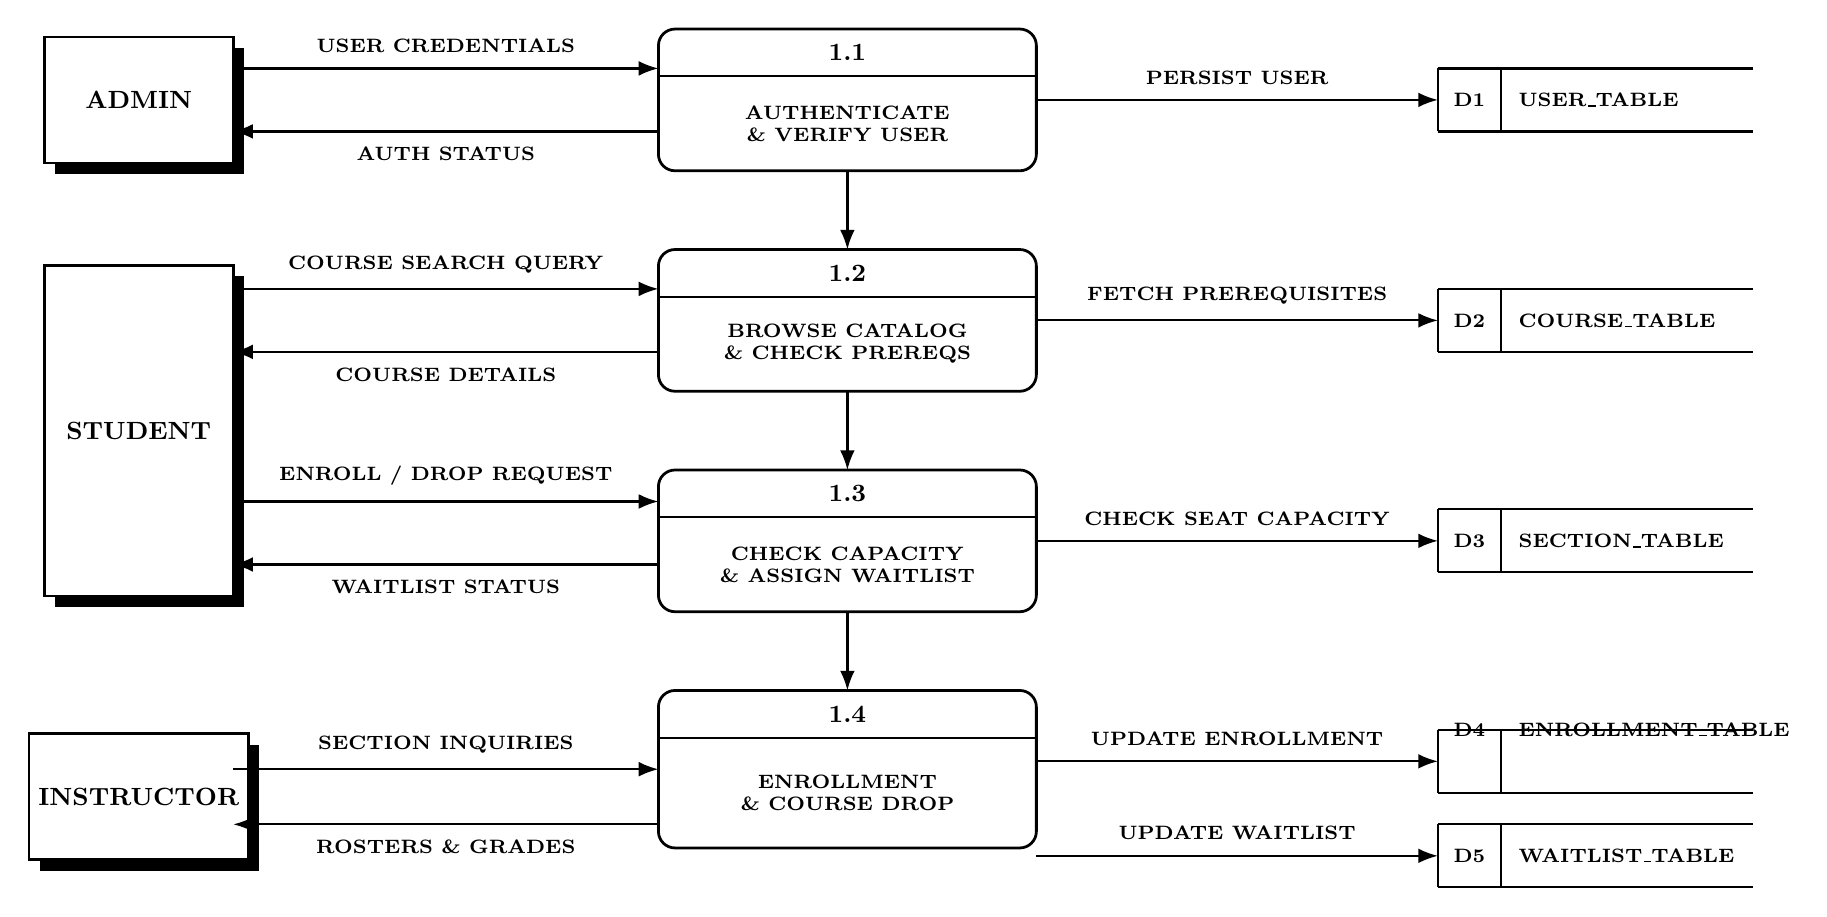
\begin{tikzpicture}[auto]
    % Sub-Process 1.1: AUTHENTICATE & VERIFY USER (Expanded to width 4.8cm)
    \draw[draw=black, line width=1pt, fill=white, rounded corners=6pt] (-2.4, 4.2) rectangle (2.4, 6.0);
    \draw[line width=0.8pt] (-2.4, 5.4) -- (2.4, 5.4);
    \node[font=\bfseries\small] at (0.0, 5.7) {1.1};
    \node[font=\bfseries\scriptsize, align=center] at (0.0, 4.8) {AUTHENTICATE\\\& VERIFY USER};

    % Sub-Process 1.2: BROWSE CATALOG & CHECK PREREQS
    \draw[draw=black, line width=1pt, fill=white, rounded corners=6pt] (-2.4, 1.4) rectangle (2.4, 3.2);
    \draw[line width=0.8pt] (-2.4, 2.6) -- (2.4, 2.6);
    \node[font=\bfseries\small] at (0.0, 2.9) {1.2};
    \node[font=\bfseries\scriptsize, align=center] at (0.0, 2.0) {BROWSE CATALOG\\\& CHECK PREREQS};

    % Sub-Process 1.3: CHECK CAPACITY & ASSIGN WAITLIST
    \draw[draw=black, line width=1pt, fill=white, rounded corners=6pt] (-2.4, -1.4) rectangle (2.4, 0.4);
    \draw[line width=0.8pt] (-2.4, -0.2) -- (2.4, -0.2);
    \node[font=\bfseries\small] at (0.0, 0.1) {1.3};
    \node[font=\bfseries\scriptsize, align=center] at (0.0, -0.8) {CHECK CAPACITY\\\& ASSIGN WAITLIST};

    % Sub-Process 1.4: PROCESS ENROLLMENT & DROP (Spacious, Cleanly bounded text)
    \draw[draw=black, line width=1pt, fill=white, rounded corners=6pt] (-2.4, -4.4) rectangle (2.4, -2.4);
    \draw[line width=0.8pt] (-2.4, -3.0) -- (2.4, -3.0);
    \node[font=\bfseries\small] at (0.0, -2.7) {1.4};
    \node[font=\bfseries\scriptsize, align=center] at (0.0, -3.7) {ENROLLMENT\\\& COURSE DROP};

    % External Entities on the Left
    \node (admin) [entity3D, minimum width=2.4cm, minimum height=1.6cm] at (-9.0, 5.1) {ADMIN};
    \node (student) [entity3D, minimum width=2.4cm, minimum height=4.2cm] at (-9.0, 0.9) {STUDENT};
    \node (instructor) [entity3D, minimum width=2.4cm, minimum height=1.6cm] at (-9.0, -3.75) {INSTRUCTOR};

    % Data Stores on the Right (Open-ended DFD notation)
    % D1: USER_TABLE
    \draw[line width=0.8pt] (7.5, 5.5) -- (11.5, 5.5);
    \draw[line width=0.8pt] (7.5, 4.7) -- (11.5, 4.7);
    \draw[line width=0.8pt] (7.5, 4.7) -- (7.5, 5.5);
    \draw[line width=0.8pt] (8.3, 4.7) -- (8.3, 5.5);
    \node[font=\bfseries\scriptsize] at (7.9, 5.1) {D1};
    \node[font=\bfseries\scriptsize, anchor=west] at (8.4, 5.1) {USER\_TABLE};

    % D2: COURSE_TABLE
    \draw[line width=0.8pt] (7.5, 2.7) -- (11.5, 2.7);
    \draw[line width=0.8pt] (7.5, 1.9) -- (11.5, 1.9);
    \draw[line width=0.8pt] (7.5, 1.9) -- (7.5, 2.7);
    \draw[line width=0.8pt] (8.3, 1.9) -- (8.3, 2.7);
    \node[font=\bfseries\scriptsize] at (7.9, 2.3) {D2};
    \node[font=\bfseries\scriptsize, anchor=west] at (8.4, 2.3) {COURSE\_TABLE};

    % D3: SECTION_TABLE
    \draw[line width=0.8pt] (7.5, -0.1) -- (11.5, -0.1);
    \draw[line width=0.8pt] (7.5, -0.9) -- (11.5, -0.9);
    \draw[line width=0.8pt] (7.5, -0.9) -- (7.5, -0.1);
    \draw[line width=0.8pt] (8.3, -0.9) -- (8.3, -0.1);
    \node[font=\bfseries\scriptsize] at (7.9, -0.5) {D3};
    \node[font=\bfseries\scriptsize, anchor=west] at (8.4, -0.5) {SECTION\_TABLE};

    % D4: ENROLLMENT_TABLE
    \draw[line width=0.8pt] (7.5, -2.9) -- (11.5, -2.9);
    \draw[line width=0.8pt] (7.5, -3.7) -- (11.5, -3.7);
    \draw[line width=0.8pt] (7.5, -3.7) -- (7.5, -2.9);
    \draw[line width=0.8pt] (8.3, -3.7) -- (8.3, -2.9);
    \node[font=\bfseries\scriptsize] at (7.9, -2.9) {D4};
    \node[font=\bfseries\scriptsize, anchor=west] at (8.4, -2.9) {ENROLLMENT\_TABLE};

    % D5: WAITLIST_TABLE
    \draw[line width=0.8pt] (7.5, -4.1) -- (11.5, -4.1);
    \draw[line width=0.8pt] (7.5, -4.9) -- (11.5, -4.9);
    \draw[line width=0.8pt] (7.5, -4.9) -- (7.5, -4.1);
    \draw[line width=0.8pt] (8.3, -4.9) -- (8.3, -4.1);
    \node[font=\bfseries\scriptsize] at (7.9, -4.5) {D5};
    \node[font=\bfseries\scriptsize, anchor=west] at (8.4, -4.5) {WAITLIST\_TABLE};

    % Admin Connections to 1.1 (Arrow span = 5.4cm)
    \draw [dfdArrow] (-7.8, 5.5) -- node[above=2pt, font=\scriptsize\bfseries, text width=4.8cm, align=center] {USER CREDENTIALS} (-2.4, 5.5);
    \draw [dfdArrow] (-2.4, 4.7) -- node[below=2pt, font=\scriptsize\bfseries, text width=4.8cm, align=center] {AUTH STATUS} (-7.8, 4.7);

    % Student Connections to 1.2 (Browse Catalog & Prereqs)
    \draw [dfdArrow] (-7.8, 2.7) -- node[above=2pt, font=\scriptsize\bfseries, text width=4.8cm, align=center] {COURSE SEARCH QUERY} (-2.4, 2.7);
    \draw [dfdArrow] (-2.4, 1.9) -- node[below=2pt, font=\scriptsize\bfseries, text width=4.8cm, align=center] {COURSE DETAILS} (-7.8, 1.9);

    % Student Connections to 1.3 (Seat Check & Waitlist)
    \draw [dfdArrow] (-7.8, 0.0) -- node[above=2pt, font=\scriptsize\bfseries, text width=4.8cm, align=center] {ENROLL / DROP REQUEST} (-2.4, 0.0);
    \draw [dfdArrow] (-2.4, -0.8) -- node[below=2pt, font=\scriptsize\bfseries, text width=4.8cm, align=center] {WAITLIST STATUS} (-7.8, -0.8);

    % Instructor Connections to 1.4 (Symmetrically aligned at y = -3.4 and y = -4.1)
    \draw [dfdArrow] (-7.8, -3.4) -- node[above=2pt, font=\scriptsize\bfseries, text width=4.8cm, align=center] {SECTION INQUIRIES} (-2.4, -3.4);
    \draw [dfdArrow] (-2.4, -4.1) -- node[below=2pt, font=\scriptsize\bfseries, text width=4.8cm, align=center] {ROSTERS \& GRADES} (-7.8, -4.1);

    % Sub-processes to Data Stores Connections (Arrow span = 5.1cm)
    \draw [dfdArrow] (2.4, 5.1) -- node[above=2pt, font=\scriptsize\bfseries, text width=4.6cm, align=center] {PERSIST USER} (7.5, 5.1);
    \draw [dfdArrow] (2.4, 2.3) -- node[above=2pt, font=\scriptsize\bfseries, text width=4.6cm, align=center] {FETCH PREREQUISITES} (7.5, 2.3);
    \draw [dfdArrow] (2.4, -0.5) -- node[above=2pt, font=\scriptsize\bfseries, text width=4.6cm, align=center] {CHECK SEAT CAPACITY} (7.5, -0.5);
    \draw [dfdArrow] (2.4, -3.3) -- node[above=2pt, font=\scriptsize\bfseries, text width=4.6cm, align=center] {UPDATE ENROLLMENT} (7.5, -3.3);
    
    % Sub-process 1.4 to D5 Waitlist Table (Direct clean horizontal arrow from 1.4 body)
    \draw [dfdArrow] (2.4, -4.5) -- node[above=2pt, font=\scriptsize\bfseries, text width=4.6cm, align=center] {UPDATE WAITLIST} (7.5, -4.5);

    % Inter-process vertical progression arrows
    \draw [dfdArrow] (0.0, 4.2) -- (0.0, 3.2);
    \draw [dfdArrow] (0.0, 1.4) -- (0.0, 0.4);
    \draw [dfdArrow] (0.0, -1.4) -- (0.0, -2.4);
\end{tikzpicture}
}
\caption{DFD Level 2: Sub-Process Decomposition of Course Registration}
\end{figure}

\newpage
\subsection{Product Functions}
The behavioral interactions of \textbf{My Student Academia} across actors are specified through UML Use Case Modeling:

\begin{figure}[H]
\centering
\resizebox{0.78\linewidth}{!}{
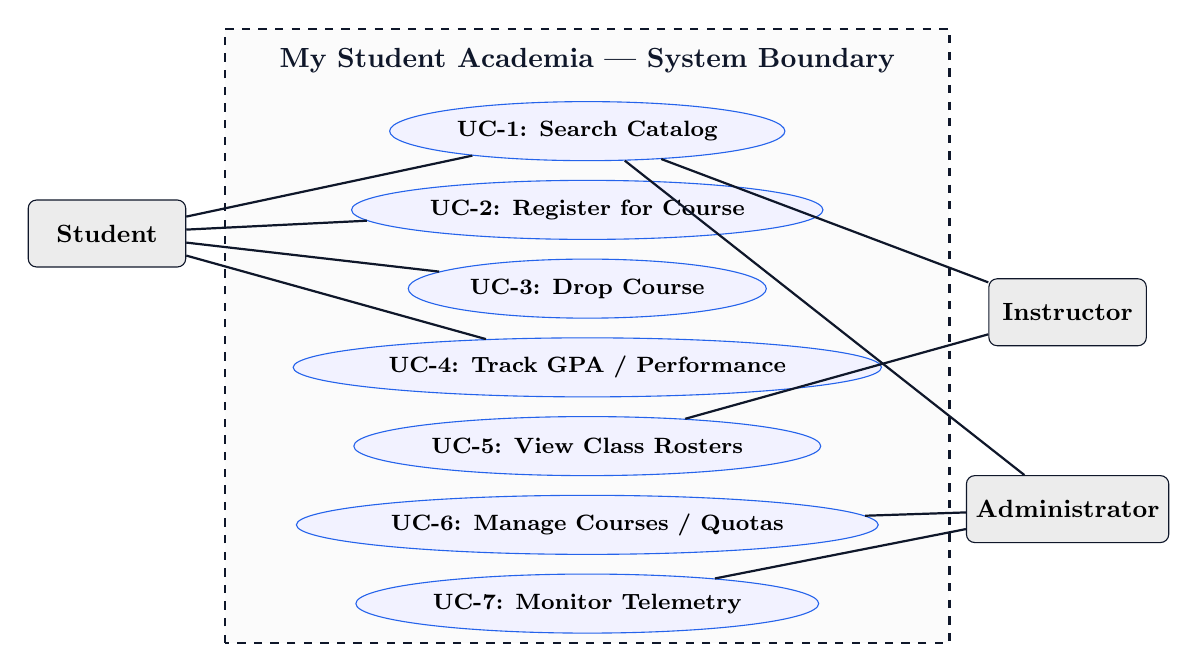
\begin{tikzpicture}[node distance=0.9cm, auto]
    % System boundary box
    \draw [draw=navyblue, thick, dashed, fill=gray!3] (0,-0.2) rectangle (9.2, 7.6);
    \node at (4.6, 7.2) {\bfseries\color{navyblue} My Student Academia --- System Boundary};
    
    % Actors
    \node (student) [actorNode] at (-1.5, 5.0) {Student};
    \node (instructor) [actorNode] at (10.7, 4.0) {Instructor};
    \node (admin) [actorNode] at (10.7, 1.5) {Administrator};
    
    % Use Cases
    \node (uc1) [usecase] at (4.6, 6.3) {UC-1: Search Catalog};
    \node (uc2) [usecase] at (4.6, 5.3) {UC-2: Register for Course};
    \node (uc3) [usecase] at (4.6, 4.3) {UC-3: Drop Course};
    \node (uc4) [usecase] at (4.6, 3.3) {UC-4: Track GPA / Performance};
    \node (uc5) [usecase] at (4.6, 2.3) {UC-5: View Class Rosters};
    \node (uc6) [usecase] at (4.6, 1.3) {UC-6: Manage Courses / Quotas};
    \node (uc7) [usecase] at (4.6, 0.3) {UC-7: Monitor Telemetry};
    
    % Associations
    \draw [thick, draw=navyblue] (student) -- (uc1);
    \draw [thick, draw=navyblue] (student) -- (uc2);
    \draw [thick, draw=navyblue] (student) -- (uc3);
    \draw [thick, draw=navyblue] (student) -- (uc4);
    
    \draw [thick, draw=navyblue] (instructor) -- (uc1);
    \draw [thick, draw=navyblue] (instructor) -- (uc5);
    
    \draw [thick, draw=navyblue] (admin) -- (uc1);
    \draw [thick, draw=navyblue] (admin) -- (uc6);
    \draw [thick, draw=navyblue] (admin) -- (uc7);
\end{tikzpicture}
}
\caption{UML Use Case Diagram}
\end{figure}

\begin{table}[H]
\centering
\small
\renewcommand{\arraystretch}{1.3}
\begin{tabularx}{\textwidth}{>{\bfseries}p{2.6cm} >{\raggedright\arraybackslash}p{4.2cm} >{\raggedright\arraybackslash}X}
\toprule
\textbf{Actor} & \textbf{Primary Use Cases} & \textbf{Operational Scope} \\
\midrule
Student & UC-1, UC-2, UC-3, UC-4 & Browse courses, check prerequisite eligibility, enroll in sections, drop courses, and track GPA standing. \\
\addlinespace
Instructor & UC-1, UC-5 & Inspect assigned course sections, review active student rosters, and monitor waitlist numbers. \\
\addlinespace
Administrator & UC-1, UC-6, UC-7 & Define course curriculum, allocate instructor sections, manage registration terms, and monitor enrollment metrics. \\
\bottomrule
\end{tabularx}
\caption{Actor-to-Use-Case Mapping Summary}
\end{table}

\subsection{User Classes and Characteristics}
\begin{enumerate}[leftmargin=1.2cm]
    \item \textbf{Students (High Frequency, Variable Technical Skill):} Primary end-users who discover courses, check prerequisites, register/drop sections, and track academic standing. Interface must be intuitive and error-tolerant.
    \item \textbf{Faculty / Instructors (Medium Frequency, Moderate Technical Skill):} Academic staff managing section rosters, grading enrollments, and monitoring waitlisted students.
    \item \textbf{Academic Administrators (Low-to-Medium Frequency, Advanced Skill):} Department heads and registrars responsible for setting up departments, creating courses, configuring capacities, and analyzing institutional telemetry.
\end{enumerate}

\subsection{Operating Environment}
\begin{itemize}[leftmargin=1.2cm]
    \item \textbf{Client Environment:} Modern web browsers supporting ECMAScript 6+ (Google Chrome 110+, Mozilla Firefox 110+, Apple Safari 16+, Microsoft Edge).
    \item \textbf{Application Server:} Node.js runtime environment (v18.0+ or v20.0+ LTS) executing Express.js application servers.
    \item \textbf{Database Management System:} Relational SQLite database engine (development) and PostgreSQL (production), managed via Prisma ORM.
    \item \textbf{Deployment Environment:} Multi-container Docker and Docker Compose environment on Linux/Windows Server hosts.
\end{itemize}

\subsection{Design and Implementation Constraints}
\begin{itemize}[leftmargin=1.2cm]
    \item \textbf{Credit Limit Constraint:} Hard constraint enforcing a strict maximum of 24 credit hours per student per semester.
    \item \textbf{Concurrency Constraint:} Seat allocations and waitlist positions must execute within ACID transactions to prevent overbooking during registration spikes.
    \item \textbf{Type Safety:} Strict static type checking across the entire full-stack codebase via TypeScript 5+.
    \item \textbf{Platform Independence:} Standard RESTful JSON communication ensuring cross-platform client compatibility.
\end{itemize}

\subsection{User Documentation}
The system provides built-in user assistance, including an interactive onboarding guide for first-time students, role-specific dashboard tooltips, and structured API documentation for backend services.

\subsection{Assumptions and Dependencies}
\begin{itemize}[leftmargin=1.2cm]
    \item \textbf{Network Connectivity:} Requires continuous HTTP/HTTPS internet connectivity for real-time catalog and registration synchronization.
    \item \textbf{Data Integrity:} Assumes student records, prerequisite histories, and departmental classifications are populated accurately in the database.
    \item \textbf{Term Window Management:} Registration operations depend on the active academic term having the \texttt{registrationOpen} flag set to \texttt{true}.
\end{itemize}

\newpage
\section{External Interface Requirements}

\subsection{User Interfaces}
The presentation layer of \textbf{My Student Academia} is designed as a responsive, modern Single-Page Application (SPA) leveraging React 18, Tailwind CSS, and Lucide React iconography. The user interface adheres to standard institutional UX design principles:

\begin{itemize}[leftmargin=1.2cm]
    \item \textbf{Global Navigation \& Status Banner:} A persistent navigation header displays user role identification, active semester indicator (e.g., \textit{Spring 2026}), registered credit counter ($\le 24$), and immediate logout access.
    \item \textbf{Visual Prerequisite Badging:} Course cards in the catalog dynamically render green badges for fulfilled prerequisites and amber/red lock badges for unmet dependencies with interactive tooltips explaining requirements.
    \item \textbf{Real-Time Toast Feedback:} All user-initiated mutations (enrollment, drop, waitlist joining, grade updates) trigger contextual non-blocking toast notifications reporting transaction success or exact validation failure reasons.
    \item \textbf{Accessibility \& Responsiveness:} Flexible CSS flexbox/grid layouts ensuring fluid rendering across desktop displays ($1920\times1080$), laptops ($1366\times768$), and tablet viewports.
\end{itemize}

\subsubsection{Key Screen Layouts \& Visual Mockups}

\begin{figure}[H]
\centering
\IfFileExists{images/student_catalog_screen.png}{
    \includegraphics[width=0.95\linewidth]{images/student_catalog_screen.png}
}{
    \resizebox{0.95\linewidth}{!}{
    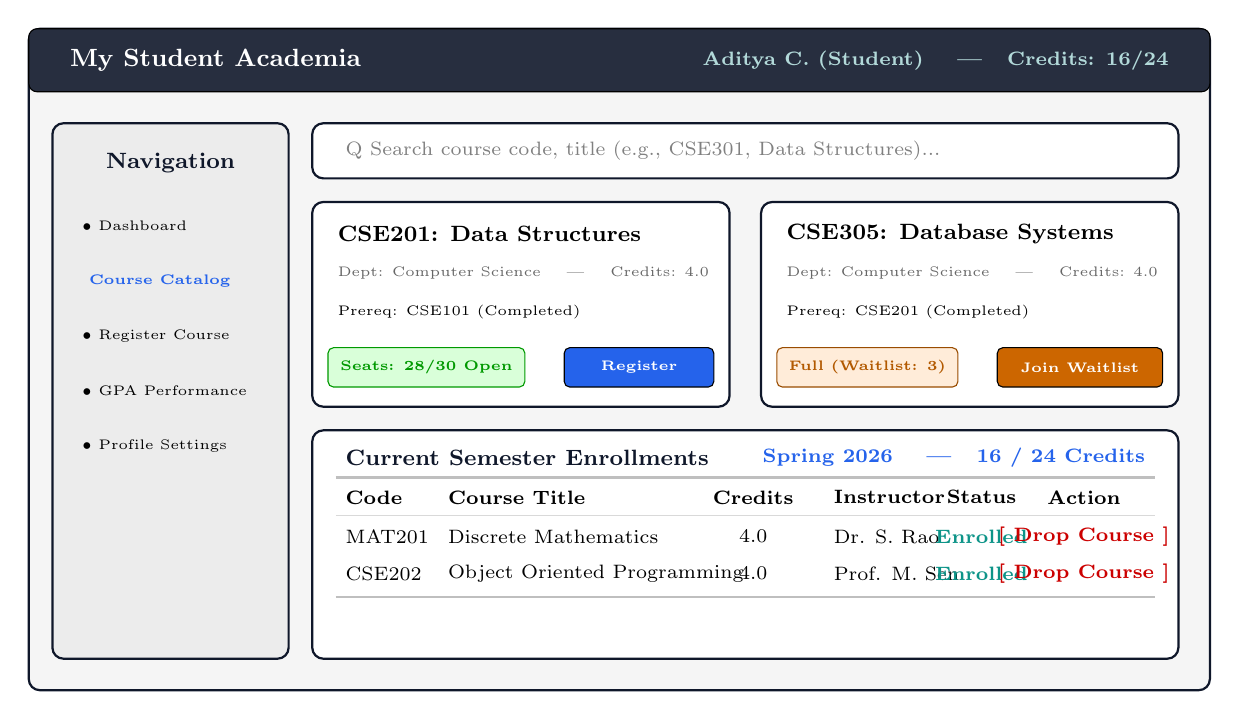
\begin{tikzpicture}[auto]
        % Window Outer Frame (Width = 15.0cm, Height = 8.4cm)
        \draw[wireframeBox, fill=gray!8] (0, 0) rectangle (15.0, 8.4);
        \draw[fill=navyblue!90, rounded corners=3pt] (0, 7.6) rectangle (15.0, 8.4);
        
        % Header with non-overlapping dedicated left and right anchors
        \node[text=white, font=\small\bfseries, anchor=west] at (0.4, 8.0) {My Student Academia};
        \node[text=teal!30, font=\scriptsize\bfseries, anchor=east] at (14.6, 8.0) {Aditya C. (Student) \quad|\quad Credits: 16/24};

        % Sidebar
        \draw[wireframeBox, fill=gray!15] (0.3, 0.4) rectangle (3.3, 7.2);
        \node[font=\footnotesize\bfseries, color=navyblue] at (1.8, 6.7) {Navigation};
        \node[font=\tiny, anchor=west] at (0.55, 5.9) {$\bullet$ Dashboard};
        \node[font=\tiny\bfseries, anchor=west, color=accentblue] at (0.55, 5.2) {$\blacktriangleright$ Course Catalog};
        \node[font=\tiny, anchor=west] at (0.55, 4.5) {$\bullet$ Register Course};
        \node[font=\tiny, anchor=west] at (0.55, 3.8) {$\bullet$ GPA Performance};
        \node[font=\tiny, anchor=west] at (0.55, 3.1) {$\bullet$ Profile Settings};

        % Search Input Bar
        \draw[wireframeBox, fill=white] (3.6, 6.5) rectangle (14.6, 7.2);
        \node[font=\scriptsize, color=gray, anchor=west] at (3.9, 6.85) {Q Search course code, title (e.g., CSE301, Data Structures)...};

        % Course Card 1 (Available)
        \draw[wireframeBox, fill=white] (3.6, 3.6) rectangle (8.9, 6.2);
        \node[font=\footnotesize\bfseries, anchor=west] at (3.8, 5.8) {CSE201: Data Structures};
        \node[font=\tiny, color=gray!80!black, anchor=west] at (3.8, 5.3) {Dept: Computer Science \quad | \quad Credits: 4.0};
        \node[font=\tiny, anchor=west] at (3.8, 4.8) {Prereq: CSE101 (Completed)};
        \draw[fill=green!15, draw=green!60!black, rounded corners=2pt] (3.8, 3.85) rectangle (6.3, 4.35);
        \node[font=\tiny\bfseries, color=green!60!black] at (5.05, 4.1) {Seats: 28/30 Open};
        \draw[fill=accentblue, rounded corners=2pt] (6.8, 3.85) rectangle (8.7, 4.35);
        \node[font=\tiny\bfseries, text=white] at (7.75, 4.1) {Register};

        % Course Card 2 (Waitlist)
        \draw[wireframeBox, fill=white] (9.3, 3.6) rectangle (14.6, 6.2);
        \node[font=\footnotesize\bfseries, anchor=west] at (9.5, 5.8) {CSE305: Database Systems};
        \node[font=\tiny, color=gray!80!black, anchor=west] at (9.5, 5.3) {Dept: Computer Science \quad | \quad Credits: 4.0};
        \node[font=\tiny, anchor=west] at (9.5, 4.8) {Prereq: CSE201 (Completed)};
        \draw[fill=orange!15, draw=orange!60!black, rounded corners=2pt] (9.5, 3.85) rectangle (11.8, 4.35);
        \node[font=\tiny\bfseries, color=orange!70!black] at (10.65, 4.1) {Full (Waitlist: 3)};
        \draw[fill=orange!80!black, rounded corners=2pt] (12.3, 3.85) rectangle (14.4, 4.35);
        \node[font=\tiny\bfseries, text=white] at (13.35, 4.1) {Join Waitlist};

        % Bottom Registered Enrollments Container Box (3.6 to 14.6)
        \draw[wireframeBox, fill=white] (3.6, 0.4) rectangle (14.6, 3.3);
        
        % Split Header (Left Title and Right Badge)
        \node[font=\footnotesize\bfseries, color=navyblue, anchor=west] at (3.9, 2.95) {Current Semester Enrollments};
        \node[font=\scriptsize\bfseries, color=accentblue, anchor=east] at (14.3, 2.95) {Spring 2026 \quad|\quad 16 / 24 Credits};
        
        % Native Vector Table Inside Box
        \draw[draw=gray!50, line width=0.8pt] (3.9, 2.7) -- (14.3, 2.7);
        \node[font=\scriptsize\bfseries, anchor=west] at (3.9, 2.45) {Code};
        \node[font=\scriptsize\bfseries, anchor=west] at (5.2, 2.45) {Course Title};
        \node[font=\scriptsize\bfseries, anchor=center] at (9.2, 2.45) {Credits};
        \node[font=\scriptsize\bfseries, anchor=west] at (10.1, 2.45) {Instructor};
        \node[font=\scriptsize\bfseries, anchor=center] at (12.1, 2.45) {Status};
        \node[font=\scriptsize\bfseries, anchor=center] at (13.4, 2.45) {Action};
        \draw[draw=gray!30, line width=0.5pt] (3.9, 2.22) -- (14.3, 2.22);
        
        % Row 1
        \node[font=\scriptsize, anchor=west] at (3.9, 1.95) {MAT201};
        \node[font=\scriptsize, anchor=west] at (5.2, 1.95) {Discrete Mathematics};
        \node[font=\scriptsize, anchor=center] at (9.2, 1.95) {4.0};
        \node[font=\scriptsize, anchor=west] at (10.1, 1.95) {Dr. S. Rao};
        \node[font=\scriptsize\bfseries, color=accentteal, anchor=center] at (12.1, 1.95) {Enrolled};
        \node[font=\scriptsize\bfseries, color=red!80!black, anchor=center] at (13.4, 1.95) {[ Drop Course ]};
        
        % Row 2
        \node[font=\scriptsize, anchor=west] at (3.9, 1.48) {CSE202};
        \node[font=\scriptsize, anchor=west] at (5.2, 1.48) {Object Oriented Programming};
        \node[font=\scriptsize, anchor=center] at (9.2, 1.48) {4.0};
        \node[font=\scriptsize, anchor=west] at (10.1, 1.48) {Prof. M. Sen};
        \node[font=\scriptsize\bfseries, color=accentteal, anchor=center] at (12.1, 1.48) {Enrolled};
        \node[font=\scriptsize\bfseries, color=red!80!black, anchor=center] at (13.4, 1.48) {[ Drop Course ]};
        \draw[draw=gray!50, line width=0.8pt] (3.9, 1.18) -- (14.3, 1.18);
    \end{tikzpicture}
    }
}
\caption{UI Mockup 1: Student Course Discovery \& Registration Interface}
\end{figure}

\begin{figure}[H]
\centering
\IfFileExists{images/instructor_admin_screen.png}{
    \includegraphics[width=0.95\linewidth]{images/instructor_admin_screen.png}
}{
    \resizebox{0.95\linewidth}{!}{
    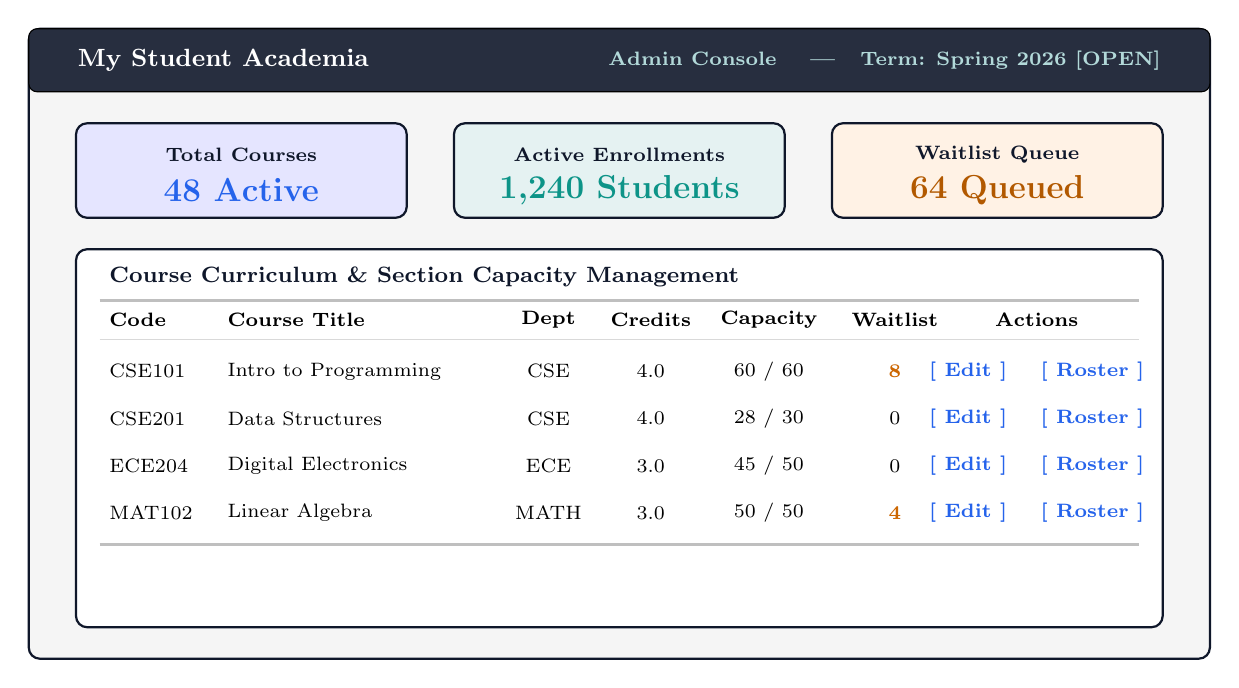
\begin{tikzpicture}[auto]
        % Window Outer Frame (Width = 15.0cm, Height = 8.0cm)
        \draw[wireframeBox, fill=gray!8] (0, 0) rectangle (15.0, 8.0);
        \draw[fill=navyblue!90, rounded corners=3pt] (0, 7.2) rectangle (15.0, 8.0);
        
        % Header with non-overlapping dedicated left and right anchors
        \node[text=white, font=\small\bfseries, anchor=west] at (0.5, 7.6) {My Student Academia};
        \node[text=teal!30, font=\scriptsize\bfseries, anchor=east] at (14.5, 7.6) {Admin Console \quad|\quad Term: Spring 2026 [OPEN]};

        % Summary KPI Cards (Evenly Spaced 3 Columns)
        \draw[wireframeBox, fill=blue!10] (0.6, 5.6) rectangle (4.8, 6.8);
        \node[font=\scriptsize\bfseries, color=navyblue] at (2.7, 6.4) {Total Courses};
        \node[font=\large\bfseries, color=accentblue] at (2.7, 5.95) {48 Active};

        \draw[wireframeBox, fill=teal!10] (5.4, 5.6) rectangle (9.6, 6.8);
        \node[font=\scriptsize\bfseries, color=navyblue] at (7.5, 6.4) {Active Enrollments};
        \node[font=\large\bfseries, color=accentteal] at (7.5, 5.95) {1,240 Students};

        \draw[wireframeBox, fill=orange!10] (10.2, 5.6) rectangle (14.4, 6.8);
        \node[font=\scriptsize\bfseries, color=navyblue] at (12.3, 6.4) {Waitlist Queue};
        \node[font=\large\bfseries, color=orange!70!black] at (12.3, 5.95) {64 Queued};

        % Management Table Box (Width = 14.4 - 0.6 = 13.8cm, Height = 5.2 - 0.4 = 4.8cm)
        \draw[wireframeBox, fill=white] (0.6, 0.4) rectangle (14.4, 5.2);
        
        % Table Box Title
        \node[font=\footnotesize\bfseries, color=navyblue, anchor=west] at (0.9, 4.85) {Course Curriculum \& Section Capacity Management};
        
        % Native Vector Table inside Admin Box
        \draw[draw=gray!50, line width=0.8pt] (0.9, 4.55) -- (14.1, 4.55);
        \node[font=\scriptsize\bfseries, anchor=west] at (0.9, 4.3) {Code};
        \node[font=\scriptsize\bfseries, anchor=west] at (2.4, 4.3) {Course Title};
        \node[font=\scriptsize\bfseries, anchor=center] at (6.6, 4.3) {Dept};
        \node[font=\scriptsize\bfseries, anchor=center] at (7.9, 4.3) {Credits};
        \node[font=\scriptsize\bfseries, anchor=center] at (9.4, 4.3) {Capacity};
        \node[font=\scriptsize\bfseries, anchor=center] at (11.0, 4.3) {Waitlist};
        \node[font=\scriptsize\bfseries, anchor=center] at (12.8, 4.3) {Actions};
        \draw[draw=gray!30, line width=0.5pt] (0.9, 4.05) -- (14.1, 4.05);
        
        % Row 1
        \node[font=\scriptsize, anchor=west] at (0.9, 3.65) {CSE101};
        \node[font=\scriptsize, anchor=west] at (2.4, 3.65) {Intro to Programming};
        \node[font=\scriptsize, anchor=center] at (6.6, 3.65) {CSE};
        \node[font=\scriptsize, anchor=center] at (7.9, 3.65) {4.0};
        \node[font=\scriptsize, anchor=center] at (9.4, 3.65) {60 / 60};
        \node[font=\scriptsize\bfseries, color=orange!80!black, anchor=center] at (11.0, 3.65) {8};
        \node[font=\scriptsize\bfseries, color=accentblue, anchor=center] at (12.8, 3.65) {[ Edit ] \quad [ Roster ]};
        
        % Row 2
        \node[font=\scriptsize, anchor=west] at (0.9, 3.05) {CSE201};
        \node[font=\scriptsize, anchor=west] at (2.4, 3.05) {Data Structures};
        \node[font=\scriptsize, anchor=center] at (6.6, 3.05) {CSE};
        \node[font=\scriptsize, anchor=center] at (7.9, 3.05) {4.0};
        \node[font=\scriptsize, anchor=center] at (9.4, 3.05) {28 / 30};
        \node[font=\scriptsize, anchor=center] at (11.0, 3.05) {0};
        \node[font=\scriptsize\bfseries, color=accentblue, anchor=center] at (12.8, 3.05) {[ Edit ] \quad [ Roster ]};
        
        % Row 3
        \node[font=\scriptsize, anchor=west] at (0.9, 2.45) {ECE204};
        \node[font=\scriptsize, anchor=west] at (2.4, 2.45) {Digital Electronics};
        \node[font=\scriptsize, anchor=center] at (6.6, 2.45) {ECE};
        \node[font=\scriptsize, anchor=center] at (7.9, 2.45) {3.0};
        \node[font=\scriptsize, anchor=center] at (9.4, 2.45) {45 / 50};
        \node[font=\scriptsize, anchor=center] at (11.0, 2.45) {0};
        \node[font=\scriptsize\bfseries, color=accentblue, anchor=center] at (12.8, 2.45) {[ Edit ] \quad [ Roster ]};
        
        % Row 4
        \node[font=\scriptsize, anchor=west] at (0.9, 1.85) {MAT102};
        \node[font=\scriptsize, anchor=west] at (2.4, 1.85) {Linear Algebra};
        \node[font=\scriptsize, anchor=center] at (6.6, 1.85) {MATH};
        \node[font=\scriptsize, anchor=center] at (7.9, 1.85) {3.0};
        \node[font=\scriptsize, anchor=center] at (9.4, 1.85) {50 / 50};
        \node[font=\scriptsize\bfseries, color=orange!80!black, anchor=center] at (11.0, 1.85) {4};
        \node[font=\scriptsize\bfseries, color=accentblue, anchor=center] at (12.8, 1.85) {[ Edit ] \quad [ Roster ]};
        \draw[draw=gray!50, line width=0.8pt] (0.9, 1.45) -- (14.1, 1.45);
    \end{tikzpicture}
    }
}
\caption{UI Mockup 2: Administrator Curriculum Control \& Quota Telemetry}
\end{figure}


\subsection{Hardware Interfaces}
The hardware interface specifications define physical deployment and client execution requirements:
\begin{itemize}[leftmargin=1.2cm]
    \item \textbf{Client Hardware:} Standard Personal Computers, Workstations, and Laptops equipped with an x86-64 or ARM processor (minimum 1.6 GHz dual-core CPU), at least 2 GB RAM, and display resolutions of $1024\times768$ pixels or higher. Standard input devices (keyboard, mouse, trackpad) are supported.
    \item \textbf{Host Server Hardware:} Application host server with minimum quad-core CPU (2.4 GHz+), 8 GB RAM, and high-speed Solid State Storage (SSD) for relational database transaction processing.
    \item \textbf{Network Hardware:} Ethernet Network Interface Cards (NIC) or Wi-Fi (802.11ac/ax) controllers with sustained broadband bandwidth ($\ge 1\text{ Mbps}$).
\end{itemize}

\subsection{Software Interfaces}
\textbf{My Student Academia} interfaces with standard runtime libraries, relational database systems, and full-stack runtime layers:
\begin{table}[H]
\centering
\small
\renewcommand{\arraystretch}{1.3}
\begin{tabularx}{\textwidth}{>{\bfseries}p{3.2cm} >{\bfseries}p{3.2cm} >{\raggedright\arraybackslash}X}
\toprule
\textbf{Component} & \textbf{Version / Standard} & \textbf{Interaction \& Service Description} \\
\midrule
React Runtime & React 18.x + Vite & Client-side DOM manipulation, reactive state hooks, virtual DOM rendering. \\
Node.js Runtime & Node.js 18.x / 20.x LTS & Asynchronous event-driven server execution, HTTP request processing. \\
Express.js Framework & Express 4.x & RESTful API routing, middleware execution, request payload validation. \\
Prisma ORM & Prisma 5.x & Type-safe database queries, schema migrations, transactional seat locking. \\
Database Engine & SQLite 3 / PostgreSQL 15 & ACID-compliant data persistence for users, terms, sections, and waitlists. \\
Operating System & Linux / Win 11 / macOS & Host OS environment supporting Node.js daemon and container execution. \\
\bottomrule
\end{tabularx}
\caption{Software Interfaces and Runtime Dependencies}
\end{table}

\subsection{Communications Interfaces}
All communications between clients and the server tier are governed by standardized web networking protocols:
\begin{itemize}[leftmargin=1.2cm]
    \item \textbf{Transport Protocol:} Hypertext Transfer Protocol Secure (HTTPS) over Transport Layer Security (TLS 1.2 / TLS 1.3) utilizing standard TCP/IP port 443.
    \item \textbf{Data Interchange Format:} RESTful JavaScript Object Notation (\texttt{application/json}) payload encapsulation for all API queries and command mutations.
    \item \textbf{Authentication Headers:} JSON Web Tokens (JWT) or Session Identity Bearer tokens passed via HTTP \texttt{Authorization: Bearer <token>} headers.
    \item \textbf{Cross-Origin Resource Sharing (CORS):} Strict CORS configuration restricting API access exclusively to trusted institutional domain origins.
\end{itemize}

\newpage
\section{System Features}

\subsection{User Authentication \& Role-Based Access Control}

\subsubsection{Description and Priority}
The Authentication subsystem handles user identity verification, password hashing, session issuance, and role entitlement routing. \\
\textbf{Priority:} High ($E$). Benefit: 9/9, Penalty: 9/9, Cost: 4/9, Risk: 3/9.

\subsubsection{Stimulus/Response Sequences}
\begin{enumerate}[leftmargin=1.2cm]
    \item \textbf{Stimulus:} User submits email and password on the \texttt{/auth} portal.
    \item \textbf{Response:} System queries database, verifies password hash with bcrypt, issues session credentials, and redirects user to their designated portal (\texttt{/dashboard}, \texttt{/instructor}, or \texttt{/admin}).
    \item \textbf{Stimulus:} User attempts to access an unauthorized route (e.g., student accessing \texttt{/admin}).
    \item \textbf{Response:} Identity Guard intercepts request and issues a \texttt{403 Forbidden} redirect to \texttt{/dashboard}.
\end{enumerate}

\subsubsection{Functional Requirements}
\begin{itemize}[leftmargin=1.2cm]
    \item \textbf{REQ-AUTH-1:} The system shall authenticate user credentials using salted bcrypt password hashes.
    \item \textbf{REQ-AUTH-2:} The system shall support role-based segregation for \textbf{Student}, \textbf{Instructor}, and \textbf{Administrator} accounts.
    \item \textbf{REQ-AUTH-3:} The system shall terminate active sessions upon user logout and revoke client tokens.
\end{itemize}

\subsection{Course Catalog Discovery \& Prerequisite Verification}

\subsubsection{Description and Priority}
Provides multi-attribute search, departmental filtering, credit breakdown, and interactive prerequisite graph validation for all active course offerings. \\
\textbf{Priority:} High ($E$). Benefit: 9/9, Penalty: 8/9, Cost: 3/9, Risk: 2/9.

\subsubsection{Stimulus/Response Sequences}
\begin{enumerate}[leftmargin=1.2cm]
    \item \textbf{Stimulus:} Student types search criteria or selects a department filter on \texttt{/catalog}.
    \item \textbf{Response:} System filters matching course records and renders sections with real-time seat counts.
    \item \textbf{Stimulus:} Student clicks on a course card to inspect details.
    \item \textbf{Response:} System checks the student's completed course history against required prerequisite IDs and displays an eligibility indicator.
\end{enumerate}

\subsubsection{Functional Requirements}
\begin{itemize}[leftmargin=1.2cm]
    \item \textbf{REQ-CAT-1:} The system shall query active course offerings filtered by title, code, department, or credits.
    \item \textbf{REQ-CAT-2:} The system shall compute prerequisite compliance by verifying prior \textit{ENROLLED}/\textit{COMPLETED} records with passing grades.
    \item \textbf{REQ-CAT-3:} The system shall display live section quotas, enrolled counts, and waitlist queue depths.
\end{itemize}

\subsection{Automated Course Enrollment \& Credit Ceiling Guard}

\subsubsection{Description and Priority}
The central business validation engine executing course enrollment transactions, enforcing duplicate prevention, validating prerequisite satisfaction, and checking the 24-credit semester ceiling. \\
\textbf{Priority:} High ($E$). Benefit: 9/9, Penalty: 9/9, Cost: 5/9, Risk: 4/9.

\subsubsection{Stimulus/Response Sequences}
\begin{enumerate}[leftmargin=1.2cm]
    \item \textbf{Stimulus:} Student clicks ``Register'' on section \texttt{CSE201-A}.
    \item \textbf{Response:} Backend initiates validation transaction:
    \begin{itemize}
        \item Checks if student is already enrolled in \texttt{CSE201} $\to$ if yes, aborts with duplicate warning.
        \item Checks $\text{Current Credits} + 4.0 \le 24.0$ $\to$ if $> 24$, aborts with credit limit alert.
        \item Checks prerequisites $\to$ if unmet, aborts with prerequisite missing error.
        \item Checks available section seats $\to$ if available, inserts \textit{ENROLLED} record, increments enrollment count, updates student credits, and returns success confirmation.
    \end{itemize}
    \item \textbf{Stimulus:} Student requests course drop on an enrolled course.
    \item \textbf{Response:} System marks status as \textit{DROPPED}, deducts course credits, decrements section count, and triggers automated waitlist promotion.
\end{enumerate}

\subsubsection{Functional Requirements}
\begin{itemize}[leftmargin=1.2cm]
    \item \textbf{REQ-ENR-1:} The system shall strictly enforce a maximum ceiling of 24 credit hours per student per semester.
    \item \textbf{REQ-ENR-2:} The system shall prevent duplicate enrollments in sections of the same course within a term.
    \item \textbf{REQ-ENR-3:} The system shall execute enrollment insertions within atomic ACID database transactions.
\end{itemize}

\subsection{Dynamic Waitlist Queue \& FIFO Seat Promotion}

\subsubsection{Description and Priority}
Automates waitlist queueing when section capacities are exhausted and automatically promotes waitlisted students upon seat vacancies. \\
\textbf{Priority:} Medium ($D$). Benefit: 7/9, Penalty: 6/9, Cost: 4/9, Risk: 3/9.

\subsubsection{Stimulus/Response Sequences}
\begin{enumerate}[leftmargin=1.2cm]
    \item \textbf{Stimulus:} Student requests enrollment in a full section and selects ``Join Waitlist''.
    \item \textbf{Response:} System calculates next sequential position ($N+1$), inserts \textit{WAITING} record, and displays confirmed queue rank.
    \item \textbf{Stimulus:} An enrolled student drops the section.
    \item \textbf{Response:} Backend background worker selects Position 1 from waitlist, verifies credit ceiling ($\le 24$), transitions record to \textit{ENROLLED}, and decrements remaining waitlist ranks by 1.
\end{enumerate}

\subsubsection{Functional Requirements}
\begin{itemize}[leftmargin=1.2cm]
    \item \textbf{REQ-WTL-1:} The system shall assign sequential 1-based FIFO queue positions to waitlisted students.
    \item \textbf{REQ-WTL-2:} The system shall automatically promote the top waitlisted student when an enrolled seat is released.
\end{itemize}

\subsection{Academic Performance \& CGPA Analytics Tracking}

\subsubsection{Description and Priority}
Aggregates completed course records, calculates Semester Grade Point Average (SGPA) and Cumulative Grade Point Average (CGPA), and visualizes credit completion progress. \\
\textbf{Priority:} Medium ($D$). Benefit: 7/9, Penalty: 4/9, Cost: 3/9, Risk: 2/9.

\subsubsection{Stimulus/Response Sequences}
\begin{enumerate}[leftmargin=1.2cm]
    \item \textbf{Stimulus:} Student navigates to \texttt{/performance}.
    \item \textbf{Response:} System computes SGPA and CGPA based on credit-weighted grade points:
    $$\text{CGPA} = \frac{\sum (\text{Credit}_i \times \text{GradePoint}_i)}{\sum \text{Credit}_i}$$
    and renders semester history tables and interactive progress charts.
\end{enumerate}

\subsubsection{Functional Requirements}
\begin{itemize}[leftmargin=1.2cm]
    \item \textbf{REQ-PRF-1:} The system shall calculate GPA metrics using 10.0 scale grade-point weighting.
    \item \textbf{REQ-PRF-2:} The system shall display total completed credits against degree graduation benchmarks.
\end{itemize}

\subsection{Administrative Curriculum \& Term Management Console}

\subsubsection{Description and Priority}
Administrative interface enabling department chairpersons and registrars to create departments, configure courses, schedule sections, allocate instructors, and toggle registration windows. \\
\textbf{Priority:} High ($E$). Benefit: 9/9, Penalty: 9/9, Cost: 4/9, Risk: 3/9.

\subsubsection{Stimulus/Response Sequences}
\begin{enumerate}[leftmargin=1.2cm]
    \item \textbf{Stimulus:} Administrator creates a new course with prerequisite linkages on \texttt{/admin}.
    \item \textbf{Response:} System persists course metadata in \texttt{COURSE\_TABLE} and prerequisite IDs in \texttt{PREREQUISITE\_TABLE}.
    \item \textbf{Stimulus:} Administrator toggles registration status for Term ``Spring 2026'' to \textit{Closed}.
    \item \textbf{Response:} System locks student enrollment endpoints and displays a ``Registration Closed'' banner.
\end{enumerate}

\subsubsection{Functional Requirements}
\begin{itemize}[leftmargin=1.2cm]
    \item \textbf{REQ-ADM-1:} The system shall provide CRUD operations for departments, courses, and sections.
    \item \textbf{REQ-ADM-2:} The system shall allow administrators to open or close term registration windows globally.
    \item \textbf{REQ-ADM-3:} The system shall generate enrollment telemetry reports and capacity utilization metrics.
\end{itemize}


\newpage
\section{Other Nonfunctional Requirements}

\subsection{Performance Requirements}
\begin{itemize}[leftmargin=1.2cm]
    \item \textbf{Response Latency (NFR-PERF-1):} Under standard load, all catalog discovery, search indexing, and profile queries shall return JSON payloads within $\le 100\text{ ms}$. Mutation endpoints (course registration and dropping) shall complete within $\le 250\text{ ms}$.
    \item \textbf{High-Concurrency Capacity (NFR-PERF-2):} The system shall support a minimum of 1,000 concurrent active student sessions during peak semester enrollment windows without transaction deadlocks or seat overselling.
    \item \textbf{Database Throughput (NFR-PERF-3):} Relational database connection pooling via Prisma ORM shall maintain sub-50ms query execution times under 500 simultaneous write transactions.
\end{itemize}

\subsection{Safety Requirements}
\begin{itemize}[leftmargin=1.2cm]
    \item \textbf{Transactional Integrity \& Rollback (NFR-SAFE-1):} All multi-table mutations (decrementing open seats, inserting enrollment records, and updating student credit counts) must execute within atomic ACID transactions. If any step fails, the entire transaction shall be rolled back immediately with zero state corruption.
    \item \textbf{Automated Crash Recovery (NFR-SAFE-2):} In the event of an unhandled exception or Node.js process termination, container orchestration daemons (Docker restart policies) shall restart the application within 5 seconds without data loss.
    \item \textbf{Data Persistence \& Backup (NFR-SAFE-3):} The database tier shall execute automated point-in-time snapshots every 24 hours with Write-Ahead Logging (WAL) enabled to prevent loss of academic records.
\end{itemize}

\subsection{Security Requirements}
\begin{itemize}[leftmargin=1.2cm]
    \item \textbf{Credential Hashing (NFR-SEC-1):} User passwords shall never be stored in plaintext and must be hashed using the \texttt{bcrypt} algorithm with a minimum work factor (salt rounds) of 10.
    \item \textbf{Session Governance \& Token Security (NFR-SEC-2):} Authentication shall be enforced via cryptographically signed JSON Web Tokens (JWT) using HMAC-SHA256 (HS256) or RSA-256 algorithms with an expiry duration of 8 hours.
    \item \textbf{Injection \& Payload Sanitization (NFR-SEC-3):} The API tier shall strictly sanitize and validate all incoming request bodies using strongly typed schema parsers (Zod / TypeScript). Parameterized SQL queries generated by Prisma ORM shall eliminate SQL Injection vulnerabilities.
    \item \textbf{Transport Layer Encryption (NFR-SEC-4):} All communications across external networks shall be encrypted over HTTPS using Transport Layer Security (TLS 1.2 or TLS 1.3).
\end{itemize}

\subsection{Software Quality Attributes}
\begin{itemize}[leftmargin=1.2cm]
    \item \textbf{Availability (NFR-QUAL-1):} The system shall achieve an uptime service level objective of $\ge 99.9\%$ during designated university registration windows.
    \item \textbf{Maintainability \& Modularity (NFR-QUAL-2):} Adherence to 3-Tier Layered Architecture with strict separation between Presentation, Business Logic Controllers, and Prisma Data Mappers ensures independent component testability and low coupling.
    \item \textbf{Portability (NFR-QUAL-3):} The system shall be fully containerized using multi-stage Docker builds, ensuring deterministic deployment parity across Linux, macOS, and Windows server environments.
    \item \textbf{Usability (NFR-QUAL-4):} User interfaces shall adhere to WCAG 2.1 Level AA accessibility standards, responsive CSS grid/flexbox layouts, and clear visual color indicators for enrollment eligibility.
\end{itemize}

\subsection{Business Rules}
\begin{itemize}[leftmargin=1.2cm]
    \item \textbf{Credit Ceiling Enforcement (BR-01):} A student cannot exceed the hard limit of 24 registered credit hours in any given academic semester ($C_{\text{current}} + C_{\text{course}} \le 24$).
    \item \textbf{Prerequisite Satisfaction (BR-02):} A student is strictly barred from enrolling in advanced courses without having completed all prerequisite courses with a passing grade.
    \item \textbf{Strict FIFO Queueing (BR-03):} Waitlist placement is strictly chronological (First-In-First-Out). When a seat is vacated, the top waitlisted candidate is automatically promoted without manual intervention.
\end{itemize}

\end{document}